\subsection{CRAFT}

% First of all, to get information for the drug identification system,  the problem of text recognition must be solved. Deep learning-based text recognition models excel in this step from reality. Initially, the researchers utilize CNN to find out which pixels belonged to text characters. Then, the text is considered as a special object, and neural networks are applied to encode the input image into feature maps. These feature maps are then fed into a classifier to predict and locate text areas. Recently, the CTPN structure is proposed and it consists of three main steps: fine-scale proposals for text detection, repeated linking text proposals and side-refinement. Fig.~\ref{fig_ctpn} illustrates these steps.

% \begin{figure}
% 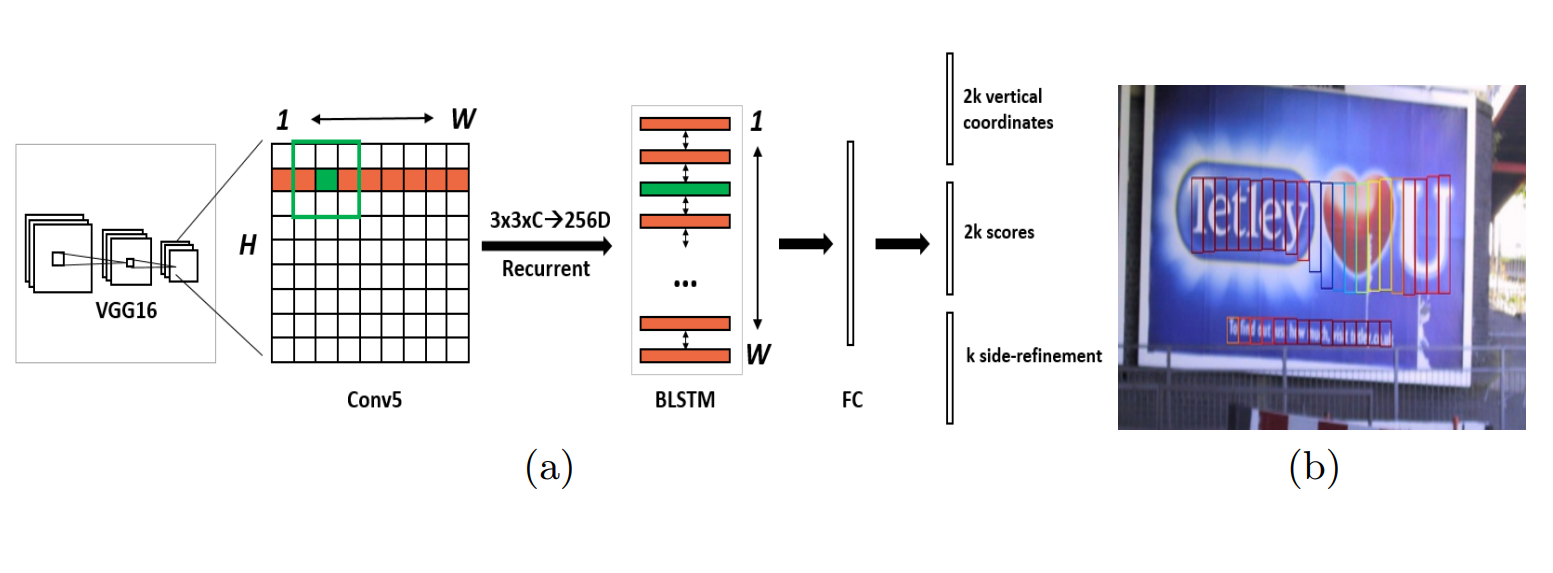
\includegraphics[width=\textwidth]{background/CTPN.png}
% \caption{The architecture of CTPN, adopted from \cite{tian2016detecting}}\label{fig_ctpn}
% \end{figure}

% In Fig.~\ref{fig_ctpn}, for text detection, the author first uses a VGG16 to extract features. Next, a sliding window slides through each location on the feature map of the final convolutional layer. Each position in the feature maps represents an attribute in the corresponding text area, which would create a "predict" that carries coordinate information and is labeled text/non-text. In fact, character detection could happen that the bounding box does not cover the entire text area because the character image has small, thin strokes or spaces between large letters. CTPN proposed a series of “fine-scale text proposals as a remedy for this problem. It is defined as a  sequence of small pieces of text that each contain one or more lines of text. An RNN layer is applied to encode this information. The results from the “predicts” would be fed into a BiLSTM network and then connected to a fully-connected layer. Integrating RNN significantly reduces false detection and obtains many text suggestions that were missed in the previous step simultaneously.  However, with the orientation-horizontal document, if the image is divided into proposals with a width of 16 pixels, it could lead to inaccurate localization or missing text areas. To further solve the outstanding problem, CTPN proceeds to estimate an additional part of the proposal on both the left and right sides (side-refinement step).


% To get information for the drug identification system, the problem of text recognition must be solved. Deep learning-based text recognition models excel in this step from reality. CRAFT is one of the most popular models used for regional text broadcasting. It detects each character area and the relationship among them. CRAFT predicts 2 metrics for each character bounding cell: (i) the region score is the probability that a given pixel is the center of the character, (ii) the affine score represents the center probability of the space among characters adjacent characters, which could be regarded as the extent to which characters are merged into one word \cite{baek2019character}. First, CRAFT generates the ground truths which are bounding boxes carrying information about the pointers and combines to give the bounds of each word. Instead of using map segmentation binaries to label each pixel individually, the author determines the encoding scale of the character center using a Gaussian heatmap. The procedure for representing the labels is as follows: 1) Prepare a 2-dimensional isotropic Gaussian map, 2) Do the computational transformation between the map and one by one character box, 3) Pack the Gaussian map into the area box. Next, with supervised learning, the characters found are broken down into small individual character sets for recognition. The images at the word level are cropped from the original image. The computational partitioning system calculates the affinity score for each region then applies an algorithm to split the characters region, thus creating bounding boxes at the character level. Eventually, it is based on the coordinates to return the character's barrier box to the origin.  Fig.1 is an illustration of CRAFT's X implementation.

To get information for the drug identification system, the problem of text recognition must be solved. In the deep learning era, CRAFT is one of the most popular models used for regional text broadcasting. It detects each character area and the relationship among them. CRAFT predicts 2 metrics for each character bounding cell: (i) the region score is the probability that a given pixel is the center of the character, (ii) the affine score represents the center probability of the space among characters adjacent characters, which could be regarded as the extent to which characters are merged into one word \cite{baek2019character}. 
\begin{figure}
\centering
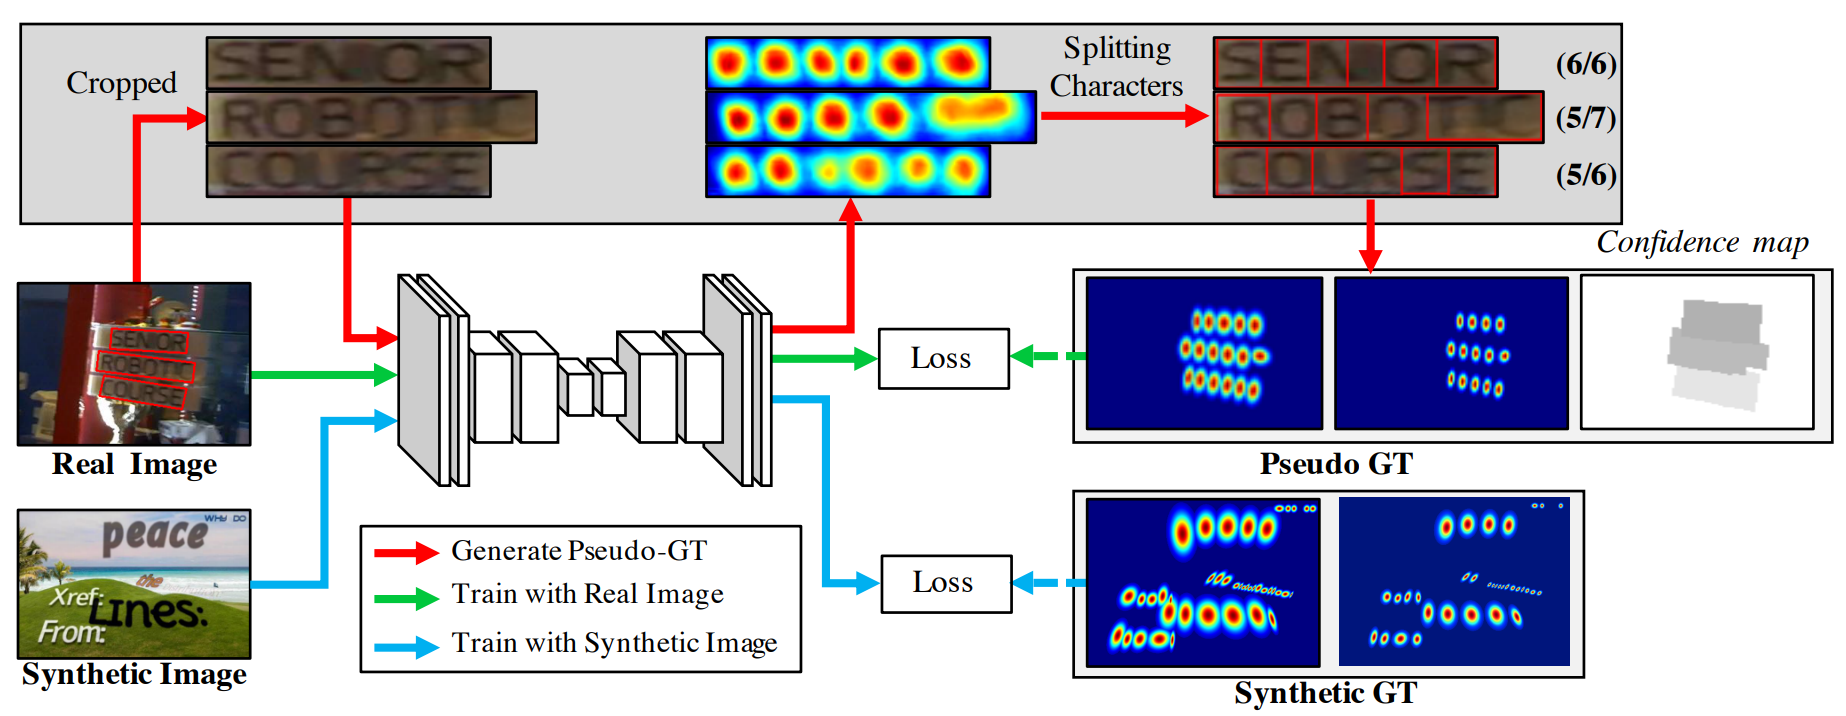
\includegraphics[width=0.7\textwidth]{background/CRAFT.png}
\caption{The architecture of CRAFT, adopted from \cite{baek2019character}}\label{fig_craft}
\end{figure}
The procedure for representing the labels is as follows. First, CRAFT generates the ground truths which are bounding boxes carrying information about the pointers and combines to give the bounds of each word. Instead of using map segmentation binaries to label each pixel individually, the author determines the encoding scale of the character center using a Gaussian heatmap. Second, with supervised learning, the characters found are broken down into small individual character sets for recognition. The images at the word level are cropped from the original image. The computational partitioning system calculates the affinity score for each region then applies an algorithm to split the characters region, thus creating bounding boxes at the character level. Eventually, it is based on the coordinates to return the character's barrier box to the origin.  Fig.1 is an illustration of CRAFT's implementation.


% In general, CTPN is capable of detecting text even in very blurry or layout-diverse images. It detects an entire text line that helps maintain text coherence. It could also recognize multilingualism without any additional processing steps. However, for tilted and skewed input images, CTPN does not perform correctly. Meanwhile, CRAFT detects each character region and the relationship between the characters then aggregates them. Instead of a bounding box around a line of characters like CTPN, CRAFT creates a bounding box for each word. The tilt, deviation of the input image almost does not affect the recognition results. However, the speed of this model is slow and might not be able to recognize single standing digits. 

% Unlike CTPN, another text detection model, which does not perform correctly for tilted and skewed input images, CRAFT detects each character region and the relationship between the characters then aggregates them that allows the tilt, deviation of the input image almost not to affect the recognition results.

% \subsection{Language model with OCR}

% Recently, many methods have been proposed to improve the accuracy of text recognition. One of them is trying to apply language models in the field of natural language processing to optical character recognition systems. In the VietOCR model, the author integrates the recognition model and the language model to produce positive results compared to traditional methods. Specifically, this model combines CNN with popular models in natural language processing such as Attention Seq2Seq, Transformer.

% In the model associated with Attention Seq2Seq---Attention OCR, since the LSTM model takes as input a 2-dimensional matrix, the feature map resulting from the CNN would be flattened before converting to the LSTM for prediction. As for the Transformer---Transformers OCR combination model, it has two principal parts Encoder and Decoder. It solves the outstanding problems of traditional technologies such as long processing time, poor concentration thanks to two special structures Multi-head attention and Positional encoding. Similar to Attention OCR, feature maps also need to be flattened before being put into position encoding. To optimize the model, VietOCR uses cross-entropy loss.

% According to the author, the accuracy of the model is stable and high even on the new data set. Using the Transformer model takes longer to execute, while its accuracy yields a negligible difference compared to another model. Seq2Seq is also more commonly used in many practical applications. In addition, VietOCR also allows retraining with new data, so this is an advantage for application developers.

\subsection{TCN}

To determine which texts are medicine in the database, we can use the Text Classification method. Convolutional Neural Network (CNN) architecture models can guarantee classification accuracy on simple strings. However, It goes terrible when texts have huge features or semantic ambiguous. To resolve, models that use Recurrent Neural Network (RNN) architecture were proposed. These models can retrieve the hidden features in sequence, which helps the model get the context in texts, like how the human brain work, making better accuracy.

Nevertheless, one drawback of RNN is the cost when dealing with extensive data. Shaojie Bai et al. \cite{bai2018empirical} proposed a new method called Temporal Convolutional Network (TCN) which is a compact version based on CNN architecture. In general, TCN stack with outstanding causal convolutions: dilated convolutions, which make TCN could learn pieces of information appeared in the past of the sequence effectively. Each output \(\textbf{y}_t\) depends on a series of \(\textbf{x}\) input, which is filtered by a parameter called \emph{filter size} on range \emph{\{0, 1, 2, …, t\}}. By measuring two-parameter \(d\) (dilation factor) and \(k\) (filter size), the model could control the suitable of deep in the sentence. With dilation, the operation of TCN brings breakthrough and recurrence similar to RNN. 
% Nevertheless, one drawback of RNN is the cost when dealing with extensive data. Shaojie Bai et al. \cite{bai2018empirical} proposed a new method called Temporal Convolutional Network (TCN) which is a compact version based on CNN architecture. In general, TCN stack with outstanding causal convolutions: dilated convolutions, which make TCN could learn pieces of information appeared in the past of the sequence effectively. Each output \(\textbf{y}_t\) depends on a series of \(\textbf{x}\) input, which is filtered by a parameter called \emph{filter size} on range \emph{\{0, 1, 2, …, t\}}. By measuring two-parameter \(d\) (dilation factor) and \(k\) (filter size), the model could control the suitable of deep in the sentence. With dilation, the operation of TCN brings breakthrough and recurrence similar to RNN. Fig.~\ref{fig_dilated} describes the architecture of the TCN model.

% \begin{figure}
% \centering
% 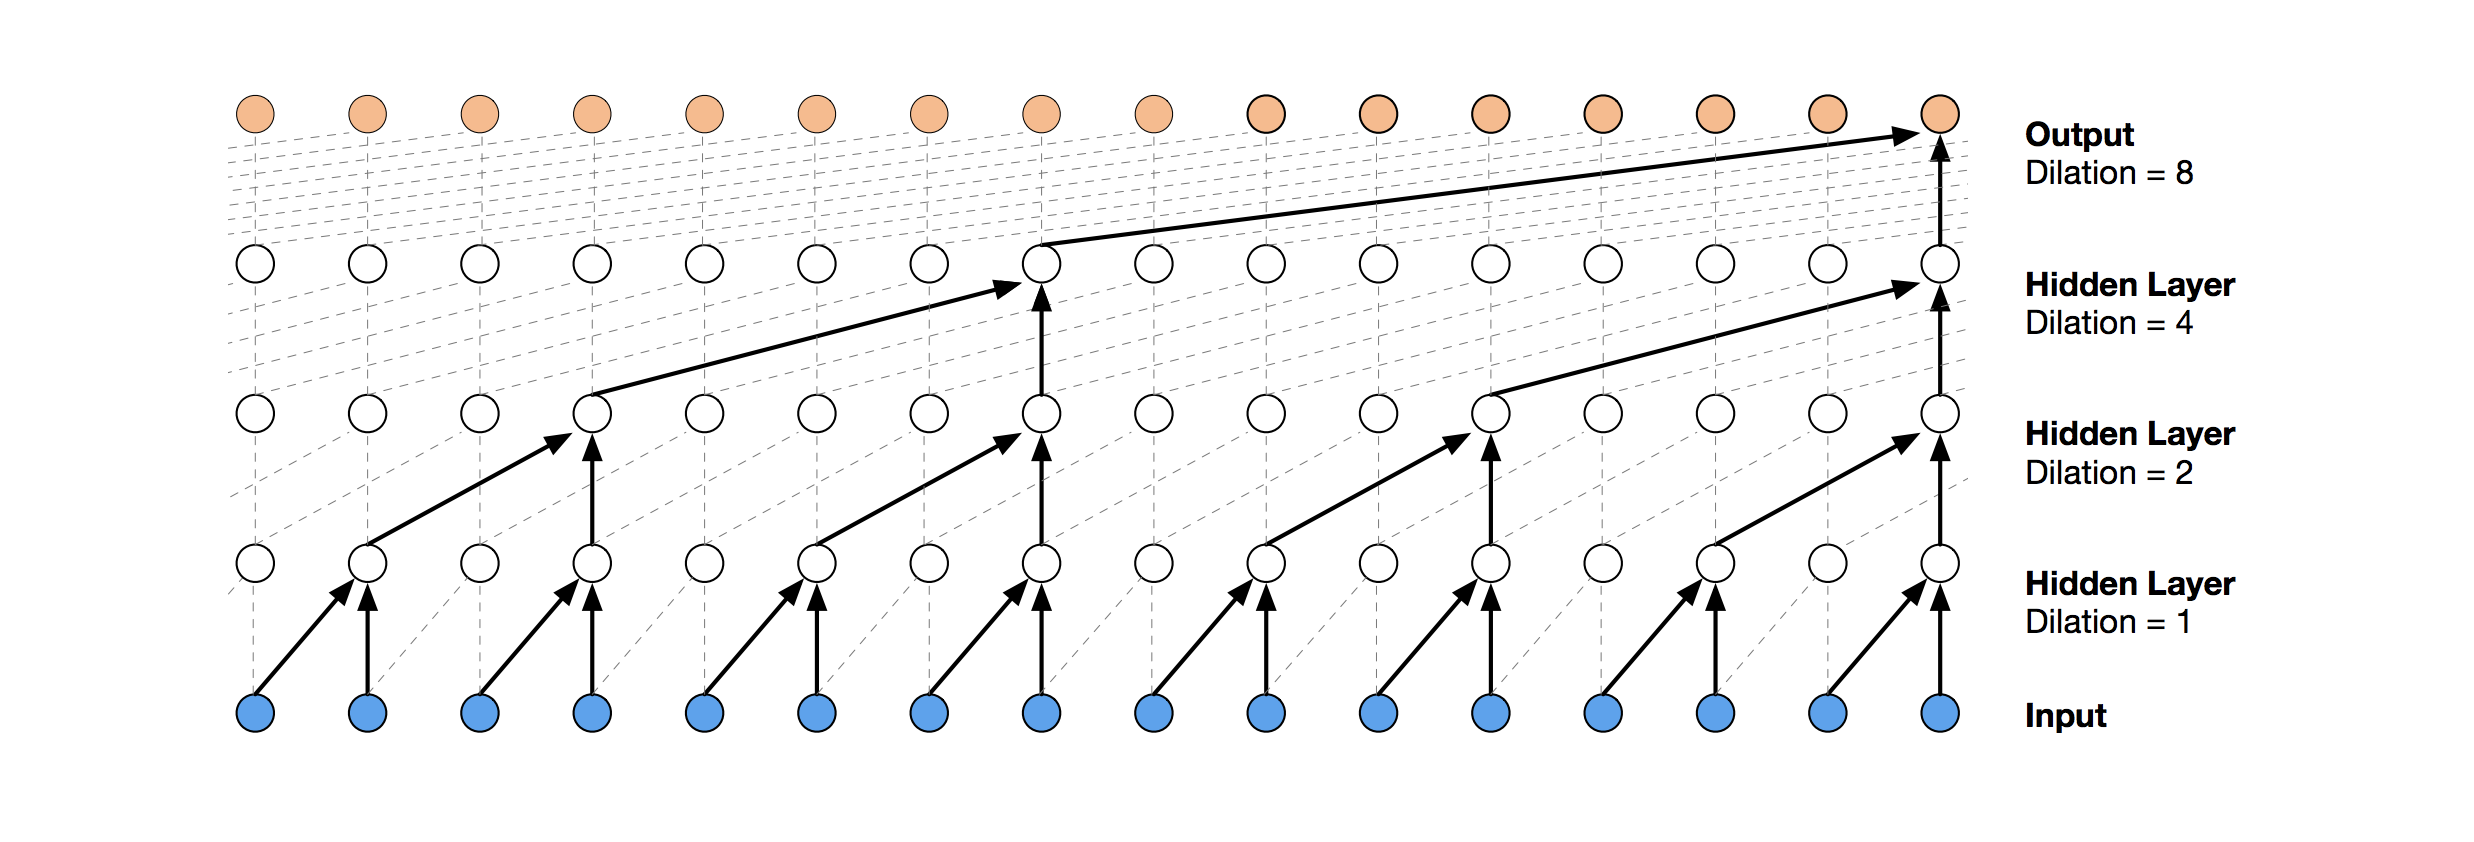
\includegraphics[width=0.8\textwidth]{background/Dilated_Conv.png}
% \caption{The architecture of TCN, adopted from \cite{TCN_architecture}}
% \label{fig_dilated}
% \end{figure}

In prescription recognition, medicine names have to be classified, which could have a unique characteristic in medical, different from other standard texts. Thus, TCN can be applied in the problem of drug name recognition and is mentioned in the proposed method section.
